\documentclass[11pt,a4paper]{article}

\usepackage{siunitx}
\usepackage{multirow}
\usepackage{subfig}

\usepackage{pgfgantt}
\usepackage{pgfgantt-custom}

\usepackage{geometry}
\usepackage{rotating}
\usepackage{hyperref}

\usepackage{setspace}
\usepackage{lineno}
\doublespacing
\linenumbers


\newcommand{\ts}{\textsuperscript}
\newcommand{\ic}{\texttt}
\newcommand\todo[1]{\textbf{TODO: #1}}
\newcommand\dom[1]{\si{#1} $\times$ \SI{#1}{km^2}}

\sisetup{detect-weight=true, detect-family=true}

\usepackage[backend=biber,style=authoryear,sorting=nyt,dashed=false]{biblatex}
\renewcommand*{\nameyeardelim}{\addcomma\space}
\addbibresource{references/references.bib} % note the .bib is required

%Wrong spellings!
%parameterization (unless part of someone else's work)
%parameterizing
%Paracon

\begin{document}

%\newgeometry{margin=2.0cm}
\newgeometry{margin=1.5cm, top=1.6cm, bottom=1.8cm}

\begin{center}
    \Large{\textbf{Monitoring Committee Report VI}}\\[0.1cm]
    \large{Mark Muetzelfeldt}\\
    \normalsize{11am on Thursday 14\ts{th} June, 2018 in 2U13}\\[0.1cm]		
    \rule{\textwidth}{0.2mm}
    \textbf{Project: }Representation of cloud field organization in a stochastic convective parametrization scheme\\
    \textbf{Monitoring Committee: }Dr Omduth Coceal and  Dr Andrew Turner\\
    \textbf{Supervisors: }Prof. Robert Plant, Prof. Peter Clark, Prof. Steven Woolnough \\
    and Dr Alison Stirling (Met Office CASE supervisor)\\
    \rule{\textwidth}{0.2mm}
\end{center}

\section{Project overview}
\label{sec:Project Overview}
% Where have I been, where am I and where am I going.

My PhD involves modifying a Convective Parametrization Scheme (CPS) in a General Circulation Model (GCM) so that it takes into account some of the effects of shear in a given grid-column. To do this, I will be classifying the shear profiles into Representative Wind Profiles (RWPs). I will then run high-resolution experiments with these RWPs as driving wind profiles, and look at certain key aspects of the cloud field such as mean cloud lifetime and bulk entrainment rate. The information derived from the high-resolution experiments, combined with a diagnosis of which RWP each grid-column fits into best, can then be used to modify the CPS under certain shear conditions. In some sense then, the organization stimulated by different dynamical conditions is being represented in the CPS. I will investigate whether running the GCM with a modified CPS has beneficial effects over regions where the organization of convection in the tropics is prevalent, e.g. over the Atlantic and West Pacific and over the Amazon and Sahel.

In MC V, one of the outstanding questions posed was `How to generate Representative Wind Profiles (RWPs)?'. I have addressed this question in the last six months to my satisfaction and am close to finalizing this stage of the analysis. This has involved running a K-means clustering algorithm to cluster wind profiles that are alike together. However, it is necessary to perform a number of steps before the profiles can be clustered. These steps are detailed in section \ref{sec:Classification of shear profiles}.

With the RWPs generated, the next step is to run high-resolution experiments with each RWP driving a Radiative-Convective Equilibrium (RCE) experiment. On starting this in March, it quickly became apparent that the simulations were developing domain-scale oscillations (DSOs). I had seen these previously (see MC IV section 2.5.1), but at the time attributed these to either using an excessively high prescribed cooling of \SI{8}{K.day^{-1}}, or to the initial $\theta$ or water vapour profiles that were used. However, I have since run experiments with low cooling rates and the initial profiles taken either from the long-term spin up of coarse simulations or as provided from the Met Office, and have observed DSOs forming. This has been a significant and hard-to-foresee setback, more detail is provided in section \ref{sec:dso}.
%, and it has had an effect on my expected finishing date (section \ref{sec:extension}).

An outstanding question for my PhD is: how to modify the CPS in light of the information from high-resolution experiments? This will involve incorporating what I have found from how cloud fields organize themselves under different shear conditions in a way that works with the CPS in use. For the Gregory-Rowntree scheme in use in the UM currently \parencite{gregory1990mass}, this could take the form of modifying the entrainment rate, based on the diagnosis of the bulk entrainment rate under different shear conditions in the high-resolution experiments. For the Plant-Craig scheme \parencite{plant2008stochastic}, this could additionally involve changing the cloud lifetime parameter based on the cloud tracking results from the high-resolution experiments. With the modifications to the CPS in place, I will be in a position to perform the idealized and global parametrized experiments tasks in my schedule (see Appendix, Fig. \ref{fig:gantt}).

\subsection{Background reading}
\label{sec:Background reading}

In preparation for writing up my work on the climatology of shear profiles in GCMs, I have been reading widely about shear and its effects on organization of convection. Fulfilling my MC V action, I have read about observations of organization, mainly in the form of Mesoscale Convective Systems (MCSs) and squall lines, and the shear profiles that cause organization. These studies come from many regions across the globe, from the Atlantic in GATE (GARP (Global Atmospheric Research Program) Atlantic Tropical Experiment) \parencite{houze1977structure, zipser1977mesoscale}, the Pacific in TOGA-COARE (Tropical Ocean Global Atmosphere - Coupled Atmosphere-Ocean Response Experiment) \parencite{jorgensen1997structure}, to continental Africa \parencite{peters1988structure} and South America \parencite{cohen1995environmental}. From these I have identified some hodographs that I can compare with those from my classification of shear work.

\section{Completed work}
\label{sec:Completed work}

\subsection{Progress overview}
\label{sec:Progress overview}

At MC V, my plan for the following six months was to follow the schedule set out in the Gantt Chart in that report. I have not managed to adhere to this, mainly because of the DSOs described in section \ref{sec:dso}. When I came across DSOs, it became a priority to work out what was the root cause of these as well as how we might be able to suppress them. There was also some slippage in the schedule before March due to the shear climatology work taking longer than I anticipated, as well as not appreciating how long it would take to organize \textit{Quo Vadis} (see section \ref{sec:Transferable skills}).

\subsection{Shear profiles classification in the UM}
\label{sec:Classification of shear profiles}
Since the last MC, I have gone from having a proof of concept working on one month of GCM output, to having a full clustering procedure that works on five years of GCM output. The GCM is the UM vn10.9, running the GA7.0 Global Atmosphere science configuration \parencite{walters2018met}. It is run for five years, from September 1988 to August 1993. In the results presented here, profiles of $u$ and $v$ are output at a number of pressure levels: \SI{950}{}, \SI{900}{}, \SI{850}{}, \SI{800}{}, \SI{700}{}, \SI{600}{}, \SI{500}{hPa} \footnote{In the final version of the analysis, 20 pressure levels from \SIrange{1000}{50}{hPa} will be used, so that information from the higher troposphere is retained in case it is needed.}. The reason that that only the low-level to mid-level shear is considered is because we hypothesize that shear at these levels is primarily responsible for organizing the convection. Only profiles that occur in the tropics, as defined by 30\si{\degree}N to 30\si{\degree}S, are considered.

The profiles are then successively filtered, normalized, have PCA applied, and are clustered until 11 RWPs have been generated. These steps are described below.

\subsubsection{Filtering}

Two filters are applied to the initial profiles. First, the grid-columns for which CAPE $<$ \SI{100}{J.kg^{-1}} are filtered out. This is to limit the analysis to only those places where convection is likely to be active, due to there being some instability in the atmosphere. Second, the maximum shear for each grid-column is calculated, and only the top 25\% of grid-columns are kept. These filtering steps are applied independently, i.e. only the intersection between the two sets of filtered grid-columns is kept.

\subsubsection{Normalization}

Two normalization steps are applied to the filtered profiles. First, the rotation is normalized: all profiles are rotated so that their wind vector at \SI{850}{hPa} is aligned in the direction of the new $u'$ axis. Given that the profiles are from near the equator, where the Coriolis force will be small, the relative rotation of the wind profiles should not matter. Second, the total magnitude of the wind at each pressure level is normalized. The magnitude of the wind at each pressure is divided by the maximum value at each pressure level, producing magnitude normalized values between 0 and 1. This effectively treats \textit{relative} differences in wind speed magnitudes between each pressure level as being equivalent when it comes to the PCA and K-means clustering steps.

\subsubsection{PCA}

Principal Component Analysis (PCA) can be used to reduce the dimensionality of a set of samples, in a way that maximizes the total explained variance when a given number of PCs are used. Reducing the number of dimensions can help the K-means clustering algorithm avoid the so-called `curse of dimensionality'. Here, the individual samples have 14 dimensions (7 each for the $u'$ and $v'$ wind). In the analysis, we choose to keep the PCs that explain over 90\% of the variance, which for this set of samples means keeping four PCs. 

\subsubsection{K-means clustering}

K-means clustering can be used to cluster samples into a user-chosen number of clusters. The algorithm used here is Lloyd's algorithm, which is described in the Appendix, section A1. The clustered RWPs can be seen in Fig. \ref{fig:RWPs}. The RWPs show some similarities with shear profiles and hodographs found in the literature (see section \ref{sec:Background reading}), this will be fully explored in my paper on shear classification in GCMs.

\begin{figure}[h!]
    \centering
    \includegraphics[height=7cm]{figs/{au197.pc_red.198809-199308.z4.ncALL_PROFILES_True_cape-shear_magrot_391137_-5_nclust-11_with_primes}.png}
    \caption{The 11 RWPs, showing the $u'$ and $v'$ components, i.e. the components normalized with respect to rotation, but not magnitude. The solid lines are the means, and the dashed lines are the 25\ts{th} and 75\ts{th} percentiles.}
    \label{fig:RWPs}
\end{figure}

The geographical distribution of the RWPs is shown in the Appendix, in Fig. \ref{fig:RWPs_geog_loc}. There are clear hotspots over certain regions: Africa, the Amazon, the West Pacific and off the east coast of Africa. These distributions will also be compared to climatologies of MCSs in my paper on shear classification.


\subsubsection{Domain-Scale Oscillations}
\label{sec:dso}

In March, when sufficient progress had been made on the RWPs, I started running some initial high-resolution (\SI{1}{km} resolution) simulations. However, it quickly became apparent that DSOs were occurring again. This sections describes DSOs, presents evidence of their existence, provides a brief explanation of why they might form, discusses some attempts at their suppression and gives the model settings to which they are sensitive or not.

% Description, results, explanation, mitigation
The DSOs can be characterized as oscillations that are present in the largest scale available to them: the domain-scale. They manifest themselves as oscillations in all the atmospheric fields that have been examined so far, e.g. $u$, $v$, $w$, surface precipitation, and surface sensible and latent heat flux. They can either form as standing or propagating waves, depending on the setup of the experiment.

In Fig. \ref{fig:hovmollers}, two Hovm{\"o}ller diagrams are shown, from which the structure and properties of the oscillations can be determined. DSOs can be seen to form after approximately \SI{1}{day}, and show oscillations in both the east-west (a) and north-south (b) directions. As time progresses, the oscillation in the east-west direction dies out, and the oscillation in the north-south direction becomes stronger. The phase speed of the oscillation is found to be \SI{13.47}{m.s^{-1}}. A single oscillation, that forms after around \SI{1}{day}, is extant for the rest of the duration of the experiment, traversing the domain approximately every \SI{5.3}{hours}.

\begin{figure}[hbt!]%
    \centering
    \subfloat[]{{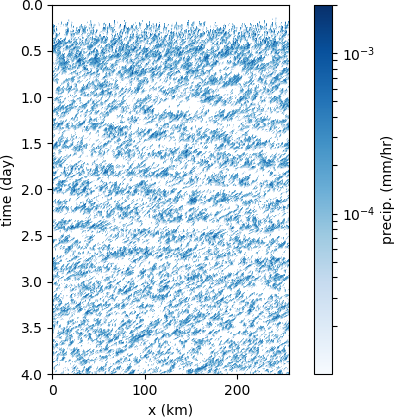
\includegraphics[height=6cm]{figs/m500_large_dom_no_wind_hovmoller_x.png}}}%
    \qquad
    \subfloat[]{{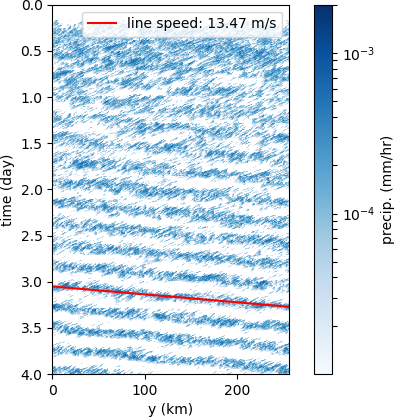
\includegraphics[height=6cm]{figs/m500_large_dom_no_wind_hovmoller_y.png}}}%
    \caption{Hovm{\"o}ller diagrams of precipitation averaged in the y-dir (a) and x-dir (b). Phase speed is marked on (b) with a red line. }%
    \label{fig:hovmollers}%
\end{figure}

Power spectra of the horizontal and vertical wind can be seen in Fig. \ref{fig:power_spectra}. In both, there is more energy in the largest scales in the y-dir (north-south), and less energy at the finest scales in the y-dir, although this is more pronounced in the vertical wind shown in subfigure (b). Both are seen to have similar gradients to a $k^{-5/3}$ line for a range of scales, indicating that there is an inertial subrange in the simulation where energy is cascading from larger length scales to smaller.

\begin{figure}[htb!]%
    \centering
    \subfloat[]{{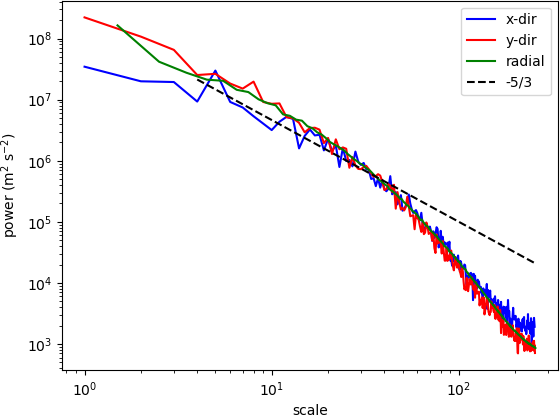
\includegraphics[width=8cm]{figs/m500_1567m_uv_mean_pow_spectrum.png}}}%
    \qquad
    \subfloat[]{{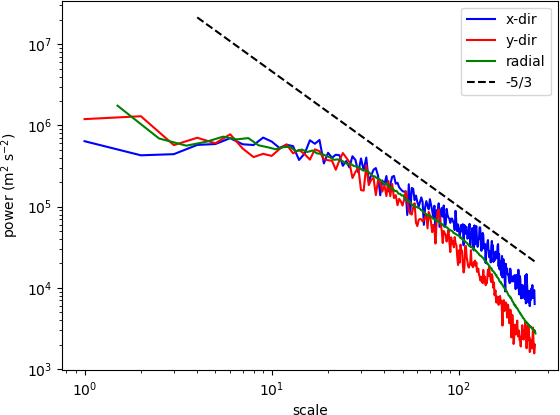
\includegraphics[width=8cm]{figs/m500_1477m_mean_pow_spectrum.png}}}%
    \caption{Power spectra in horizontal wind (a) and vertical wind (b) for a \SI{500}{m} resolution simulation, at around \SI{1477}{m} (a) and \SI{1567}{m} (b) height, averaged over 24 hourly snapshots from day 4 of the simulation. Spectra in the x-dir (blue), y-dir(red) and radially averaged (green) are shown in both subfigures. A dashed $k^{-5/3}$ line is shown in both for comparison with spectra. Scale on x-axis is in units of \SI{}{L^{-1}}, where $L$ is the domain length of \SI{256}{km}. Hence $10^0$ is the domain scale, and a value of 256 on x-axis corresponds to $2 \Delta x$ or \SI{1}{km}}%
    \label{fig:power_spectra}%
\end{figure}

We hypothesize that DSOs are convectively coupled gravity waves on the tropopause. Their phase speed is close to that of gravity waves of this type, in \cite{gill1982atmosphere} a speed of \SI{12}{m.s^{-1}} is quoted. The peaks in the $w$ field are where convection is active, and convection is suppressed in the troughs. 

The oscillations in one sense represent a physically meaningful response to the experimental setup. In a situation where there is upscale transport of energy, it must build up on the largest scale available to it, i.e. the domain-scale. However, the largest scale is determined by how we chose to setup the experiment. It is therefore not a physically meaningful scale, and so suppression of these oscillations is desirable. To do this, I have tried implementing two forms of damping: $w$ damping and $n = 1$ damping. $w$ damping consists of a Rayleigh damping term of the $w$ field at each height level in the model, with a characteristic timescale that is user settable. $n = 1$ damping involves using Fourier analysis to work out the projection of the $w$ field onto a domain-scale sinusoidal wave, and using this to damp the $w$ field. So far, $w$ damping has not had much effect, using either a \SI{6}{hour} or \SI{1}{hour} damping timescale. The $n = 1$ damping is still in the process of being implemented.

The DSOs have been found to be sensitive to some model settings, and not to others. They occur with a horizontal resolution of \SI{1}{km} or finer, but not with a resolution of \SI{2}{km}. They occur on a domain of size \dom{256}, but not on a domain of \dom{128} or smaller. They are not sensitive to the applied wind, the gravity wave sponge layer strength or depth, the forcing (between \SIrange{1.5}{2}{K.day^{-1}}), or whether geostrophic forcing or a Coriolis force is applied.

\subsection{Paper review}

I was asked to review a paper: ``Convective organization in ICON large-eddy simulations'' for QJRMS. This paper looked at the question of how to define an index of organization for convective cloud fields, and used a wavelet based approach to define one. Their index, the Wavelet Organization Index (WOI), is based on the ratio of how much power there is at large and small scales, the total amount of power at all scales, and a measure of horizontal anisotropy of the cloud field. 
% Reviewing it was a great chance for me to engage in the scientific process. I learnt about wavelets as a tool for analysis, and found some interesting papers whilst reviewing the references, such as \cite{weniger2017spatial} and \cite{wong2016spectral}. 
My recommendation was for ``Major revision with reconsideration'' as in my opinion there were too many unanswered questions and there were far too many typographical errors.

\section{Future work}
\label{sec:Future work}

\subsection{Shear profiles classification and climatology in the UM}
\label{sec:Shear climatology in the UM}

Finishing off the shear classification work in June will be a priority. The work is almost complete, although I would like to add one extra piece of analysis: examining the seasonal dependence of the RWPs. With this work done, I will then be in a good position to write the paper describing this technique after my paternity leave. It will also provide the RWPs for my high-resolution experiments.

\subsubsection{Domain-Scale Oscillations}
\label{sec:dso_future}
I am mindful that I have spent a lot of time working on the DSOs. The high-resolution modelling is an integral part of my PhD, and sorting out this issue provides the best route to performing these experiments. However, I cannot work on this indefinitely, and if I cannot make progress soon I will have to fall back on a contingency plan. My proposal is that I carry on with the $n = 1$ damping, combined with perhaps extending this and the $w$ damping to all wind fields. If I have not managed to suppress the DSOs by the end of August, I will fall back on my contingency plan. This will involve either running \SI{2}{km} experiments, or running on a smaller domain where DSOs are not so readily created, or a combination of the two. Each of these has drawbacks. Running at a coarser resolution will not resolve the convection as well as I would like, ideally I would be running at \SI{500}{m} or higher, although many previous studies have been done with \SI{2}{km} resolution, e.g. \cite{tompkins2017organization}. Running on a smaller domain will make simulating organized features such as squall lines, which can have lengths of over \SI{100}{km}, more difficult.

\subsection{High-resolution idealized modelling}
\label{sec:High-resolution idealized modelling}

Once the RWPs have been generated, and having made a decision about how best to deal with the DSOs, I will be in a position to perform the high-resolution experiments. This will involve running an experiment for each of the RWPs, and running experiments for linearly scaled shear profiles, as was done for the companion paper to MC IV, using an otherwise identical model setup. The analysis from the MC IV companion paper will then be run, supplemented by the cloud tracking work described in MC V.

\subsection{Parametrized simulations}
\label{sec:Parametrized simulations}

Once the high-resolution experiments have been run, I can start making changes to the CPS in the UM. I have done work on the technical aspects of this, however implementing the changes will require a degree of experimentation. Running idealized parametrized experiments consists of making modifications to the CPS and running an idealized RCE experiment that is equivalent to the high-resolution RCE experiments. This can be used to verify that the changes I have made are producing the correct results compared to the high-resolution `truth'. The global experiments involve running a setup similar to GA7.0 but with a modified CPS, and investigating the changes to the behaviour of the GCM with respect to a control run.

There is a combined total of \SI{6}{months} in my schedule for the idealized and global parametrized tasks.  However, there is scope for some flexibility in how long I spend on each, and there is also some flexibility as to the nature of the idealized experiments. Jian-Feng Gu (one of Robert Plant's post-doctoral researchers) has run idealized parametrized simulations, so I will be liaising with him to find out how he has progressed with these. There is the possibility of changing the idealized experiments to single column model experiments as well, should the coupling between the CPS and the dynamics in the idealized experiments prove to be troublesome. I would like to discuss this in MC VII, as hopefully I will have had time to do some initial experimentation into the idealized parametrized runs by then.

\subsection{Writing}
\label{sec:Writing}

I have \SI{10}{months} of thesis writing in my schedule. This overlaps with the parametrized simulations, and my plan is to be writing up chapters as I am doing this work. My writing during this time will be lower intensity, increasing as I complete the work. There is also some time at the end to write up a paper of the high-resolution experiments. 
% There will of course be significant overlap between both papers I am planning on writing and thesis chapters.

\section{Extension to funding}
\label{sec:extension}

The unforeseen issue of the DSOs, combined with the fact that I had significant difficulties with moisture conservation in the idealized UM when I started using it, means that I will be asking for more than the \SI{3.5}{years} that it would be expected to take for someone who did six assessed modules. 
I now expect to finish by the 1\ts{st} of September, 2019, which is five months after the finished date I put forward in MC V. Bearing in mind that this also includes a month of paternity leave (2 weeks statutory and 2 weeks annual holiday), and the extra time spent diagnosing and mitigating the DSO issue, I think this represents a realistic and achievable plan for the remainder of my PhD. It also includes an extra month for writing a paper at the end of my PhD; I have checked with Clare Watt that budgeting for this is acceptable.

\section{Training record}
\label{sec:Training record}

I completed my third RRDP, going to a course on ``How to write a paper''. This course provided an overview of how to publish a scientific paper, from considering which journals are most suited to the paper, to how to respond to reviewer comments. It will come in useful in the near future.

\subsection{Posters, presentations and conferences}
\label{sec:presentations}

I presented a poster on clustering of wind profiles at the Met Office in Exeter during the Met Office Academic Partnership (MOAP) poster presentations. This poster was the precursor to the poster that I presented at EGU, and helped me work out how best to present the clustering procedure and results.

I presented my work on clustering of wind profiles in a talk in Mesoscale Group, where I got some useful feedback on extra analysis to consider.  I presented what I have found regarding DSOs in a short talk in the ParaCon meeting, after which there was a good discussion on what we could try to further investigate the phenomenon.

\subsubsection{EGU conference 2018}

I attended the EGU conference in Vienna from the 9\ts{th} to the 13\ts{th} of April. This exposed me to the breadth and depth of research being carried out in atmospheric science and beyond. 
%The session that was most directly relevant for me was on ``Atmospheric convection'', where I saw some interesting talks on self-aggregation and the organization of convection.
I presented a poster on ``Clustering wind profiles to identify shear conditions in climate models'', which was a chance to showcase my research outside of the department and led to a few useful conversations about how the analysis could expanded upon. The poster sessions also provided ample opportunity to get an in-depth run through of another scientist's work, and I had many fruitful talks with people and made some useful connections.

\subsection{Transferable skills}
\label{sec:Transferable skills}

As co-chair of the PGR forum, I have represented the PhD students to the department. Last term, this involved helping to speed up the relocation of a room of PhD students in Harry Pitt who were unhappy with their room, as there was a noisy ventilation unit in it. I also organized \textit{Quo Vadis}, making sure that 18 students got their presentations to us on time. I chaired one of the sessions, where I gained some experience of keeping speakers to a strict \SI{12}{minute} time limit.

\printbibliography[title={References}]

\newpage
\section*{Appendix}

\renewcommand\thefigure{A.\arabic{figure}}
\setcounter{figure}{0}    
\subsection*{PhD Timetable}

\begin{figure}[htp!]
    \begin{ganttchart}[vgrid, hgrid, y unit chart=0.75cm, 
MC/.style={milestone/.append style={shape=circle},
}]{1}{23} 
    \gantttitle{2017}{2}
    \gantttitle{2018}{12}
    \gantttitle{2019}{9} \\
    \gantttitle{N}{1}
    \gantttitle{D}{1}
    \gantttitle{J}{1}
    \gantttitle{F}{1}
    \gantttitle{M}{1}
    \gantttitle{A}{1}
    \gantttitle{M}{1}
    \gantttitle{J}{1}
    \gantttitle{J}{1}
    \gantttitle{A}{1}
    \gantttitle{S}{1}
    \gantttitle{O}{1}
    \gantttitle{N}{1}
    \gantttitle{D}{1}
    \gantttitle{J}{1}
    \gantttitle{F}{1}
    \gantttitle{M}{1}
    \gantttitle{A}{1}
    \gantttitle{M}{1}
    \gantttitle{J}{1} 
    \gantttitle{J}{1} 
    \gantttitle{A}{1}
    \gantttitle{S}{1} \\
    \ganttmilestone[MC, milestone left shift=0.2,milestone right shift=-0.2]{Monitoring committees}{2} 
    \ganttmilestone[MC, milestone left shift=0.2,milestone right shift=-0.2]{}{8} 
    \ganttmilestone[MC, milestone left shift=0.2,milestone right shift=-0.2]{}{14}  
    \ganttmilestone[MC, milestone left shift=0.2,milestone right shift=-0.2]{}{20}  \\
    \ganttbar{Paternity leave}{9}{9} \\
    \ganttbar{GCM shear climatology}{2}{4} 
    \ganttbar{}{8}{8} 
    \ganttmilestone{}{8} \\
    \ganttbar{High-resolution modelling}{5}{5} 
    \ganttbar{}{11}{13} 
    \ganttmilestone{}{13} \\
    \ganttbar{DSO investigation}{5}{8}
    \ganttbar{}{10}{10}
    \ganttmilestone{}{10} \\
    \ganttbar{GCM shear paper writing}{5}{5} 
    \ganttbar{}{11}{12} 
    \ganttmilestone{}{12} \\
    \ganttbar{High-resolution paper writing}{21}{22} 
    \ganttmilestone{}{22} \\
    \ganttbar{Idealized parametrized}{14}{16} \\
    \ganttbar{Global parametrized}{17}{19} 
    \ganttmilestone{}{19} \\
    \ganttbar{Thesis writing}{12}{21} 
    \ganttmilestone{}{21} 
    \drawverticalline{7}{Now}
\end{ganttchart}
\caption{MC V6 Gantt chart showing remaining timetable and tasks. Milestones shown as diamonds. Thesis writing will ramp up starting in Q3 this year. The proposed finish date is 1\ts{st} September, 2019.}
\label{gantt}
\end{figure}

\begin{figure}[htp!]
    \centering
    \includegraphics[width=470px]{figs/{au197.pc_red.198809-199308.z4.ncPROFILES_GEOG_LOC_True_cape-shear_magrot_391137_-5_nclust-11_cropped}.png}
    \caption{Hodograph of each RWP (left) and Heatmaps of the geographical distribution of each of the RWPs (right). In the hodographs, 1 is the lowest pressure level (\SI{950}{hPa}), and 7 is the highest (\SI{500}{hPa})}
    \label{fig:RWPs_geog_loc}
\end{figure}

\subsection*{A1 - Lloyd's algorithm}

If it is decided to split the samples into $N$ clusters, $N$ of the samples are chosen at random. These become the cluster centres. Every other sample is then put into a cluster, based on which of the cluster centres it is nearest to (in a Euclidean sense). The mean of each cluster can then be calculated, and these are set as the new cluster centres. This process is iterated, until there is a small change in the cluster centres' location (less than some small pre-defined threshold), when the algorithm terminates.

\newpage
\subsection*{Training record}
\subsubsection*{Year 1}

\begin{itemize}
  \item RRDP: Intermediate/Advanced \LaTeX\ (4/11/2015)
  \item RRDP: You and your supervisor (11/11/2015)
  \item RRDP: Quality assurance in research (18/11/2015)
  \item RRDP (equivalent): UM Training (16-18/12/2015)
  \item RRDP (equivalent): Preparing to teach: Introduction to teaching and learning (26/1/2016)
  \item Preparing to teach: Marking and feedback (26/1/2016)
  \item Preparing to teach: Laboratory demonstrating and leading small groups (27/1/2016)
  \item MONC Training course (9-10/2/2016)
  \item RRDP (equivalent): Fairbrother Lecture ``A slippery situation: melting ice in Antarctica'' (4/5/2016)
  \item ECMWF Parametrization of subgrid physical processes (16-20/5/2016)
\end{itemize}

\subsubsection*{Year 2}

\begin{itemize}
  \item RRDP: Managing your research project (17/11/2016)
  \item RRDP: How to write a thesis (24/1/2017)
  \item SCENARIO Data Assimilation Course (14-15/2/2017)
  \item RRDP: Presentation skills (7/3/2017)
  \item Software Development for scientists (8/3/2017, 28-29/3/2017)
\end{itemize}

\subsubsection*{Year 3}

\begin{itemize}
  \item NCAS Climate Modelling Summer School: demonstrating Numerical Methods for Hilary Weller (11-15/11/2017)
  \item CASE Met Office Placement (30/10/2017 - 24/11/2017)
  \item RRDP: Open access for research publications (27/11/2017)
  \item RRDP: Introduction to impact (30/11/2017)
  \item RRDP: How to write a paper (10/5/2018)
\end{itemize}

\subsection*{Talks and conferences attended}

\begin{itemize}
  \item Climate Change 2013: The physical science basis. Institute of Physics (2/2014)
  \item Dame Julia Slingo: Taking the planet into uncharted territory: What climate models can tell us about the future (9/2014)
  \item SCENARIO NERC DTP Conference (9/6/2015)
  \item Climate Change in the run-up to the Paris conference: what has Physics got to say? (6/11/2015)
  \item RMetS talk: The risk and vulnerability of Europe to severe convective storms (6/4/2016)
  \item ParaCon plenary 1 in Reading (27-28/6/2016)
  \item RMetS debate: What will make the public and politicians take climate change more seriously? (5/10/2016)
  \item RMetS talks: Come Rain or Come Shine (19/10/2016)
  \item COP22 Marrakech: Remote participation (11/11/2016)
  \item ParaCon plenary 2 in Leeds (6-7/12/2016)
  \item RMetS talks: Chaos and Confidence in Weather Forecasting (14/12/2016)
  \item ParaCon plenary 3 in Cambridge (3-4/7/2017)
  \item The Future of Cumulus Parametrization, Delft University of Technology (10-14/7/2017)
  \item ParaCon plenary 4 in Exeter (18-19/12/2017)
  \item EGU 2018 in Vienna (8-13/4/2018)
  \item (planned) ParaCon plenary 5 in Reading (27-28/6/2018)
\end{itemize}

\subsection*{Talks and conferences presented at}

\begin{itemize}
  \item Presentation: ``Effects of Shear on Cloud Field Organization''. \textit{Quo Vadis}, University of Reading (1/2/2017)
  \item Poster: ``Effects of Shear on Cloud Field Organization''. Met Office Academic Partnership (MOAP), Met Office, Exeter (22/2/2017)
  \item Poster: ``Effects of Vertical Shear on Cloud Field Organization and Variability''. The Future of Cumulus Parametrization, Delft University of Technology (10-14/7/2017)
  \item Poster: ``Effects of Vertical Shear on Cloud Field Organization and Variability''. PhD Poster Session (21/9/2017)
  \item Poster: ``Clustering wind profiles to identify shear conditions in climate models''. Met Office Academic Partnership (MOAP), Met Office, Exeter (15/2/2018)
  \item Poster: ``Clustering wind profiles to identify shear conditions in climate models''. EGU Conference (9/4/2018)
  \item (planned) Presentation: ``Domain Scale Oscillations in the idealized UM''. ParaCon plenary Reading (27-28/6/2018)
\end{itemize}

\end{document}
